

\section{Generated GUI of VDM Models}
\label{sec:guibuilder}

Overture has a feature for controlling a VDM model with a generic GUI,
automatically generated from the model~\cite{nunes&11}.\footnote{This feature is currently only
available for VDM++ models.} The generated GUI follows the same
principles as discussed in \autoref{sec:gui}. But rather than the user having to
implement the GUI himself, everything is automatically generated.
  In order to use the Generated GUI feature, simply launch the model
as a VDM  GUI configuration (see \autoref{fig:guibuilder-launch}).


\begin{figure}[!ht]
\begin{center}
  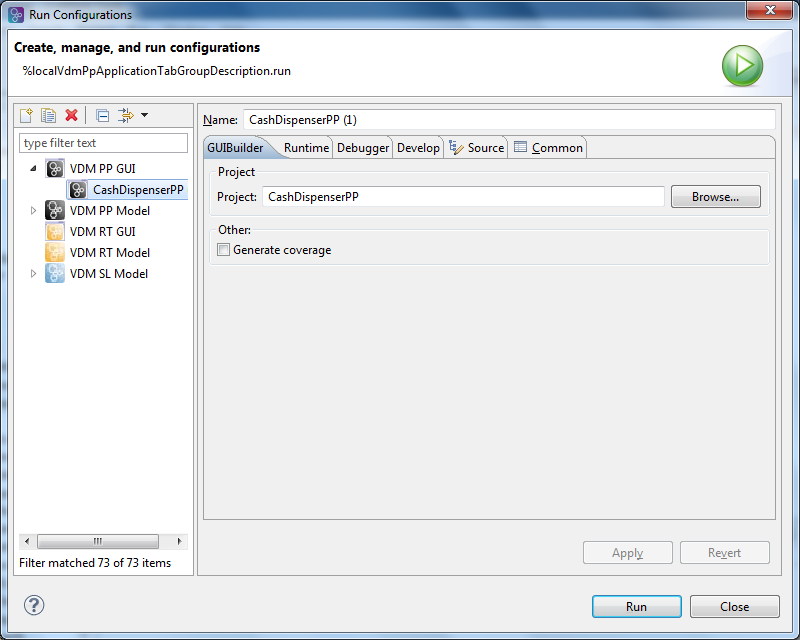
\includegraphics[width=\textwidth]{screenDumps/guibuilder-launch}
  \caption[labelInTOC]{VDM GUI Launch configuration}
  \label{fig:guibuilder-launch}
\end{center}
\end{figure}


Once the model has launched, the generic GUI will offer a list of all
classes allowing to create instances of each (see
\autoref{fig:guibuilder-instances}). These instances can then be selected to
inspect their state and invoke operations (see
\autoref{fig:guibuilder-account}). Any created instance or operation called will
be sent to the model, allowing to interact with it. Any responses from the
model are also shown in the GUI.


\begin{figure}[!ht]
\begin{center}
  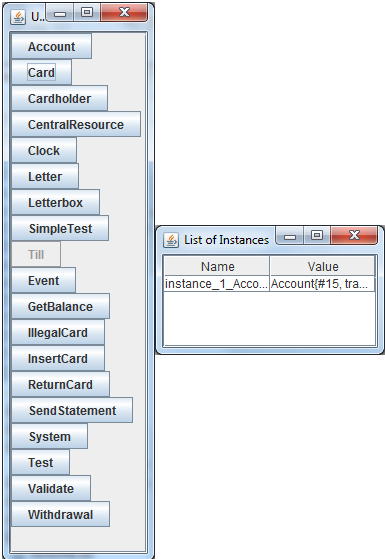
\includegraphics[width=0.45\textwidth]{screenDumps/guibuilder-instances}
  \caption[labelInTOC]{Automated GUI class list for Cash Dispenser example.}
  \label{fig:guibuilder-instances}
\end{center}
\end{figure}

\begin{figure}[!ht]
\begin{center}
  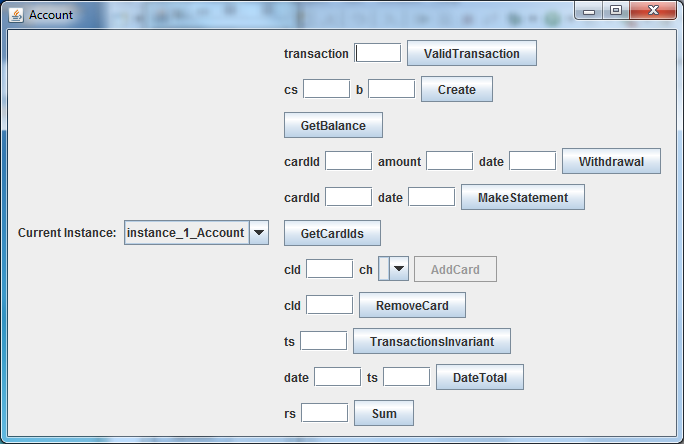
\includegraphics[width=0.45\textwidth]{screenDumps/guibuilder-account}
  \caption[labelInTOC]{Instance viewer showing the Account class.}
  \label{fig:guibuilder-account}
\end{center}
\end{figure}
